% Created 2022-12-20 mar. 10:47
% Intended LaTeX compiler: pdflatex
\documentclass[paper=a4, 12pt, DIV=12]{scrartcl}
\usepackage[utf8]{inputenc}
\usepackage[T1]{fontenc}
\usepackage{graphicx}
\usepackage{longtable}
\usepackage{wrapfig}
\usepackage{rotating}
\usepackage[normalem]{ulem}
\usepackage{amsmath}
\usepackage{amssymb}
\usepackage{capt-of}
\usepackage{hyperref}
\usepackage{minted}
\usepackage{amsfonts}
\usepackage[english]{babel}
\usepackage{bookmark}
\usepackage{xcolor}
\definecolor{pnasblue}{RGB}{0,101,165}
\hypersetup{colorlinks=true, allcolors=pnasblue}
\definecolor{bg}{rgb}{0.95,0.95,0.95}
\author{Ghislain Vieilledent\textsuperscript{\(\ast\), \ddag{}}}
\date{\today}
\title{Using the \texttt{riskmapjnr} Python module to map the deforestation risk following the JNR methodology\\\medskip
\large \textcolor{pnasblue}{Second report for FAO focused on Kenya\\ FAO budget code: TF/NFODD/TFGB110021450}}
\hypersetup{
 pdfauthor={Ghislain Vieilledent\textsuperscript{\(\ast\), \ddag{}}},
 pdftitle={Using the \texttt{riskmapjnr} Python module to map the deforestation risk following the JNR methodology},
 pdfkeywords={},
 pdfsubject={},
 pdfcreator={Emacs 28.2 (Org mode 9.5.5)}, 
 pdflang={English}}
\makeatletter
\newcommand{\citeprocitem}[2]{\hyper@linkstart{cite}{citeproc_bib_item_#1}#2\hyper@linkend}
\makeatother

\usepackage[notquote]{hanging}
\begin{document}

\maketitle

\vspace{-1cm}
\begin{center}
  $\ast$ \textbf{Correspondence to:}~ghislain.vieilledent@cirad.fr \\
  $\ddag$ \textbf{CIRAD}, UMR AMAP, F-34398 Montpellier, FRANCE \\
\end{center}
\vspace{0.25cm}

\begin{abstract}
The JNR (Jurisdictional Nested REDD+) provides a standardized approach to estimate and credit greenhouse gas (GHG) emission reductions in the framework of REDD+ (Reducing Emissions from Deforestation and Forest Degradation) programs. The JNR approach relies on a map of the deforestation risk to be able to allocate the deforestation spatially within the jurisdiction when projecting future deforestation under the reference scenario. The JNR Risk Mapping Tool presents a standardized approach to obtain this map of the deforestation risk. The methodology is based on minimal spatial information provided by the past deforestation map at the jurisdictional scale. While the methodology favors simplicity, the approach requires several computationally intensive geoprocessing steps on potentially large raster files. The \texttt{riskmapjnr} Python package we developed provides easy-to-use functions to obtain the risk map following the JNR methodology. Functions use optimized Python code that can efficiently process large raster files without memory issues. Here we provide an example of the use of the \texttt{riskmapjnr} Python package for Kenya. \textbf{The package is still under development. The code might include some errors and still need to be thoroughly tested}. A first stable version (v1.0) of the package will be released at the end of the year 2022. As a consequence, \textbf{these preliminary results should be interpreted with caution}.
\end{abstract}

\vspace{0.25cm}
\begin{center}

\includegraphics[width=0.86\textwidth]{images/partners_logos.png}\enlargethispage{2\baselineskip}
\end{center}
\newpage
\tableofcontents
\newpage
\listoffigures
\newpage

\section{Introduction}
\label{sec:orge729f14}

\subsection{Context}
\label{sec:org4cd718c}

In the forest sector, programs to mitigate GHG emissions across entire national or subnational jurisdictions (called \href{https://redd.unfccc.int/}{REDD+} programs, i.e. programs aiming at Reducing Emissions from Deforestation and Forest Degradation) can be accounted for and credited using a jurisdictional-scale framework called \href{https://verra.org/project/jurisdictional-and-nested-redd-framework/}{JNR} (Jurisdictional and Nested REDD+). JNR integrates government-led and project-level REDD+ activities and establishes a clear pathway for subnational- and project-level activities to be incorporated within broader REDD+ programs. The JNR framework ensures all projects and other reducing emissions from deforestation and degradation activities in a given jurisdiction are developed using consistent baselines and crediting approaches. They mitigate the risk of ``leakage'', i.e. the displacement of emission-causing activities to areas outside the project boundary, by monitoring emissions across an entire jurisdictional area. JNR is part of the \href{https://verra.org/project/vcs-program/}{VCS} (Verified Carbon Standard) program which allows certified projects to turn their greenhouse gas (GHG) emission reductions and removals into tradable carbon credits. Since its launch in 2006, the VCS program has grown into the world's largest voluntary GHG program.

The \href{https://verra.org/wp-content/uploads/2021/04/DRAFT\_JNR\_Risk\_Mapping\_Tool\_15APR2021.pdf}{JNR Risk Mapping Tool} is a ``benchmark'' methodology that provides a standardized approach for developing deforestation and forest degradation risk maps for users of the \href{https://verra.org/wp-content/uploads/2021/04/JNR\_Allocation\_Tool\_Guidance\_v4.0.pdf}{JNR Allocation Tool} in the context of JNR requirements. The methodology allows deriving a map of the deforestation (or degradation) risk based on a minimal spatial information provided by the past deforestation (or degradation) map at the jurisdictional scale. The \href{https://verra.org/wp-content/uploads/2021/04/DRAFT\_JNR\_Risk\_Mapping\_Tool\_15APR2021.pdf}{JNR Risk Mapping Tool} allows the creation of categorical and spatially static maps whose categories represent different levels of risk of deforestation or forest degradation in the validity period of the Forest Reference Emissions Level (FREL) and throughout the jurisdictional geographical boundaries. In the \href{https://verra.org/wp-content/uploads/2021/04/JNR\_Allocation\_Tool\_Guidance\_v4.0.pdf}{JNR Allocation Tool}, the level of risk determines how the jurisdictional FREL is spatially distributed to nested lower-level jurisdictional programs and projects.

\subsection{Objectives}
\label{sec:org1bc932a}

While the \href{https://verra.org/wp-content/uploads/2021/04/DRAFT\_JNR\_Risk\_Mapping\_Tool\_15APR2021.pdf}{JNR Risk Mapping Tool} methodology favors simplicity, obtaining the risk map is not straightforward. The approach requires several geoprocessing steps on raster data that can be large, i.e. covering large spatial extent (eg. national scale) at high spatial resolution (eg. 30 m). The \texttt{riskmapjnr} Python package we developed includes functions to perform these geoprocessing steps and derive a risk map on any jurisdiction and at any spatial resolution following the \href{https://verra.org/wp-content/uploads/2021/04/DRAFT\_JNR\_Risk\_Mapping\_Tool\_15APR2021.pdf}{JNR Risk Mapping Tool} methodology. The \texttt{riskmapjnr} package includes functions to:

\begin{enumerate}
\item Estimate the distance to forest edge beyond which the deforestation risk is negligible: \texttt{dist\_edge\_threshold()}.
\item Compute local deforestation rates using a moving window whose size can vary: \texttt{local\_defor\_rate()}.
\item Transform local deforestation rates into categories of deforestation risks using several slicing algorithms: \texttt{set\_defor\_cat\_zero()} and \texttt{defor\_cat()}
\item Validate maps of deforestation risk and select the map with the higher accuracy: \texttt{defrate\_per\_cat()} and \texttt{validation()}.
\end{enumerate}

The \texttt{riskmapjnr} package uses several known Python scientific packages such as \texttt{NumPy}, \texttt{SciPy}, and \texttt{Pandas} for fast matrix and vector operations and \texttt{gdal} for processing georeferenced raster data. Raster data are divided into blocks of data for in-memory processing. Such an approach allow processing large raster files with large geographical extents (e.g. country scale) and high spatial resolutions (eg. 30 m). Here we present an example of the use of the \texttt{riskmapjnr} Python package for Kenya following all the steps of the JNR methodology.

\subsection{Warnings}
\label{sec:orgecb5f77}

The \texttt{riskmapjnr}  package is still under development. The code might include some errors and still need to be thoroughly tested. A first stable version (v1.0) of the package will be released at the end of the year 2022. As a consequence, the preliminary results presented here should be interpreted with caution. Moreover, the JNR methodology is currently discussed and will be subject to changes in the coming months. Future versions of the \texttt{riskmapjnr} package should integrate these changes.

\section{Initial setup and data}
\label{sec:org9484763}

\subsection{Installation}
\label{sec:org05e8204}

You need several dependencies to run the \texttt{riskmapjnr} Python package. The best way to install the package is to create a Python virtual environment, either through \texttt{conda} (recommended) or \texttt{virtualenv}.

\begin{enumerate}
\item Using \texttt{conda} (recommended)
\label{sec:orgdd59cfb}

You first need to have \texttt{miniconda3} installed (see \href{https://docs.conda.io/en/latest/miniconda.html}{miniconda instructions}). Then, create a conda environment (see \href{https://docs.conda.io/projects/conda/en/latest/user-guide/tasks/manage-environments.html}{conda environment instructions}) and install the \texttt{riskmapjnr} package with the following commands:

\begin{minted}[breaklines=true,bgcolor=bg]{shell}
conda create --name conda-rmj -c conda-forge python=3 gdal numpy matplotlib pandas pip scipy --yes
conda activate conda-rmj
pip install riskmapjnr # For PyPI version
# pip install https://github.com/ghislainv/riskmapjnr/archive/master.zip # For GitHub dev version
# conda install -c conda-forge jupyter geopandas descartes folium --yes  # Optional additional packages
\end{minted}

To deactivate and delete the conda environment:

\begin{minted}[breaklines=true,bgcolor=bg]{shell}
conda deactivate
conda env remove --name conda-rmj
\end{minted}

\item Using \texttt{virtualenv}
\label{sec:orge8ca6ba}

You first need to have the \texttt{virtualenv} package installed (see \href{https://packaging.python.org/guides/installing-using-pip-and-virtual-environments/}{virtualenv instructions}). Then, create a virtual environment and install the \texttt{riskmapjnr} package with the following commands:

\begin{minted}[breaklines=true,bgcolor=bg]{shell}
cd ~
mkdir venvs # Directory for virtual environments
cd venvs
virtualenv --python=/usr/bin/python3 venv-rmj
source ~/venvs/venv-rmj/bin/activate
# Install numpy first
pip install numpy
# Install gdal (the correct version) 
pip install --global-option=build_ext --global-option="-I/usr/include/gdal" gdal==$(gdal-config --version)
pip install riskmapjnr # For PyPI version, this will install all other dependencies
# pip install https://github.com/ghislainv/riskmapjnr/archive/master.zip # For GitHub dev version
pip install jupyter geopandas descartes folium # Optional additional packages
\end{minted}

To deactivate and delete the virtual environment:

\begin{minted}[breaklines=true,bgcolor=bg]{shell}
deactivate
rm -R ~/venvs/venv-rmj # Just remove the repository
\end{minted}

\item Installation testing
\label{sec:org23fd74a}

You can test that the package has been correctly installed using the command \texttt{riskmapjnr} in a terminal:

\begin{minted}[breaklines=true,bgcolor=bg]{shell}
riskmapjnr
\end{minted}

This should return a short description of the \texttt{riskmapjnr} package and the version number:

\begin{minted}[breaklines=true,bgcolor=bg]{shell}
# riskmapjnr: Map of deforestation risk following JNR methodology.
# https://ecology.ghislainv.fr/riskmapjnr/
# riskmapjnr version x.x.
\end{minted}

You can also test the package executing the commands in the \href{https://ecology.ghislainv.fr/riskmapjnr/notebooks/get\_started.html}{Get started} tutorial of the \href{https://ecology.ghislainv.fr/riskmapjnr}{\texttt{riskmapjnr} website}.
\end{enumerate}

\subsection{Importing Python modules}
\label{sec:org29c2009}

We import the Python modules needed for running the analysis.

\begin{minted}[breaklines=true,bgcolor=bg]{python}
# Imports
import os
import multiprocessing as mp
import pkg_resources

import numpy as np
import matplotlib.pyplot as plt
import pandas as pd
from tabulate import tabulate

import riskmapjnr as rmj
\end{minted}

Increase the cache for GDAL to increase computational speed.

\begin{minted}[breaklines=true,bgcolor=bg]{python}
# GDAL
os.environ["GDAL_CACHEMAX"] = "1024"
\end{minted}

Set the \texttt{PROJ\_LIB} environmental variable.

\begin{minted}[breaklines=true,bgcolor=bg]{python}
os.environ["PROJ_LIB"] = os.path.join(
    "/home/ghislain/.pyenv/versions/miniconda3-latest/",
    "envs/conda-rmj/share/proj")
\end{minted}

Create a directory to save the results.

\begin{minted}[breaklines=true,bgcolor=bg]{python}
out_dir = "outputs_kenya"
rmj.make_dir(out_dir)
\end{minted}

\subsection{Forest cover change data}
\label{sec:org2e5338d}

We consider recent forest cover change data for Kenya. The raster file (\texttt{fcc123\_KEN\_101418.tif}) includes the following values: \textbf{1} for deforestation on the period 2010--2014, \textbf{2} for deforestation on the period 2014--2018, and \textbf{3} for the remaining forest in 2018. NoData value is set to \textbf{0}. The first period (2010--2014) will be used for calibration and the second period (2014--2018) will be used for validation.

\begin{minted}[breaklines=true,bgcolor=bg]{python}
fcc_file = "data/fcc123_KEN_101418.tif"
print(fcc_file)
border_file = "data/ctry_border_KEN.gpkg"
print(border_file)
\end{minted}

\begin{verbatim}
data/fcc123_KEN_101418.tif
data/ctry_border_KEN.gpkg
\end{verbatim}


We plot the forest cover change map with the \texttt{plot.fcc123()} function.

\begin{minted}[breaklines=true,bgcolor=bg]{python}
ofile = os.path.join(out_dir, "fcc123.png")
fig_fcc123 = rmj.plot.fcc123(
    input_fcc_raster=fcc_file,
    maxpixels=1e8,
    output_file=ofile,
    borders=border_file,
    linewidth=0.2,
    figsize=(5, 4), dpi=800)
ofile
\end{minted}

\begin{figure}[H]
\centering
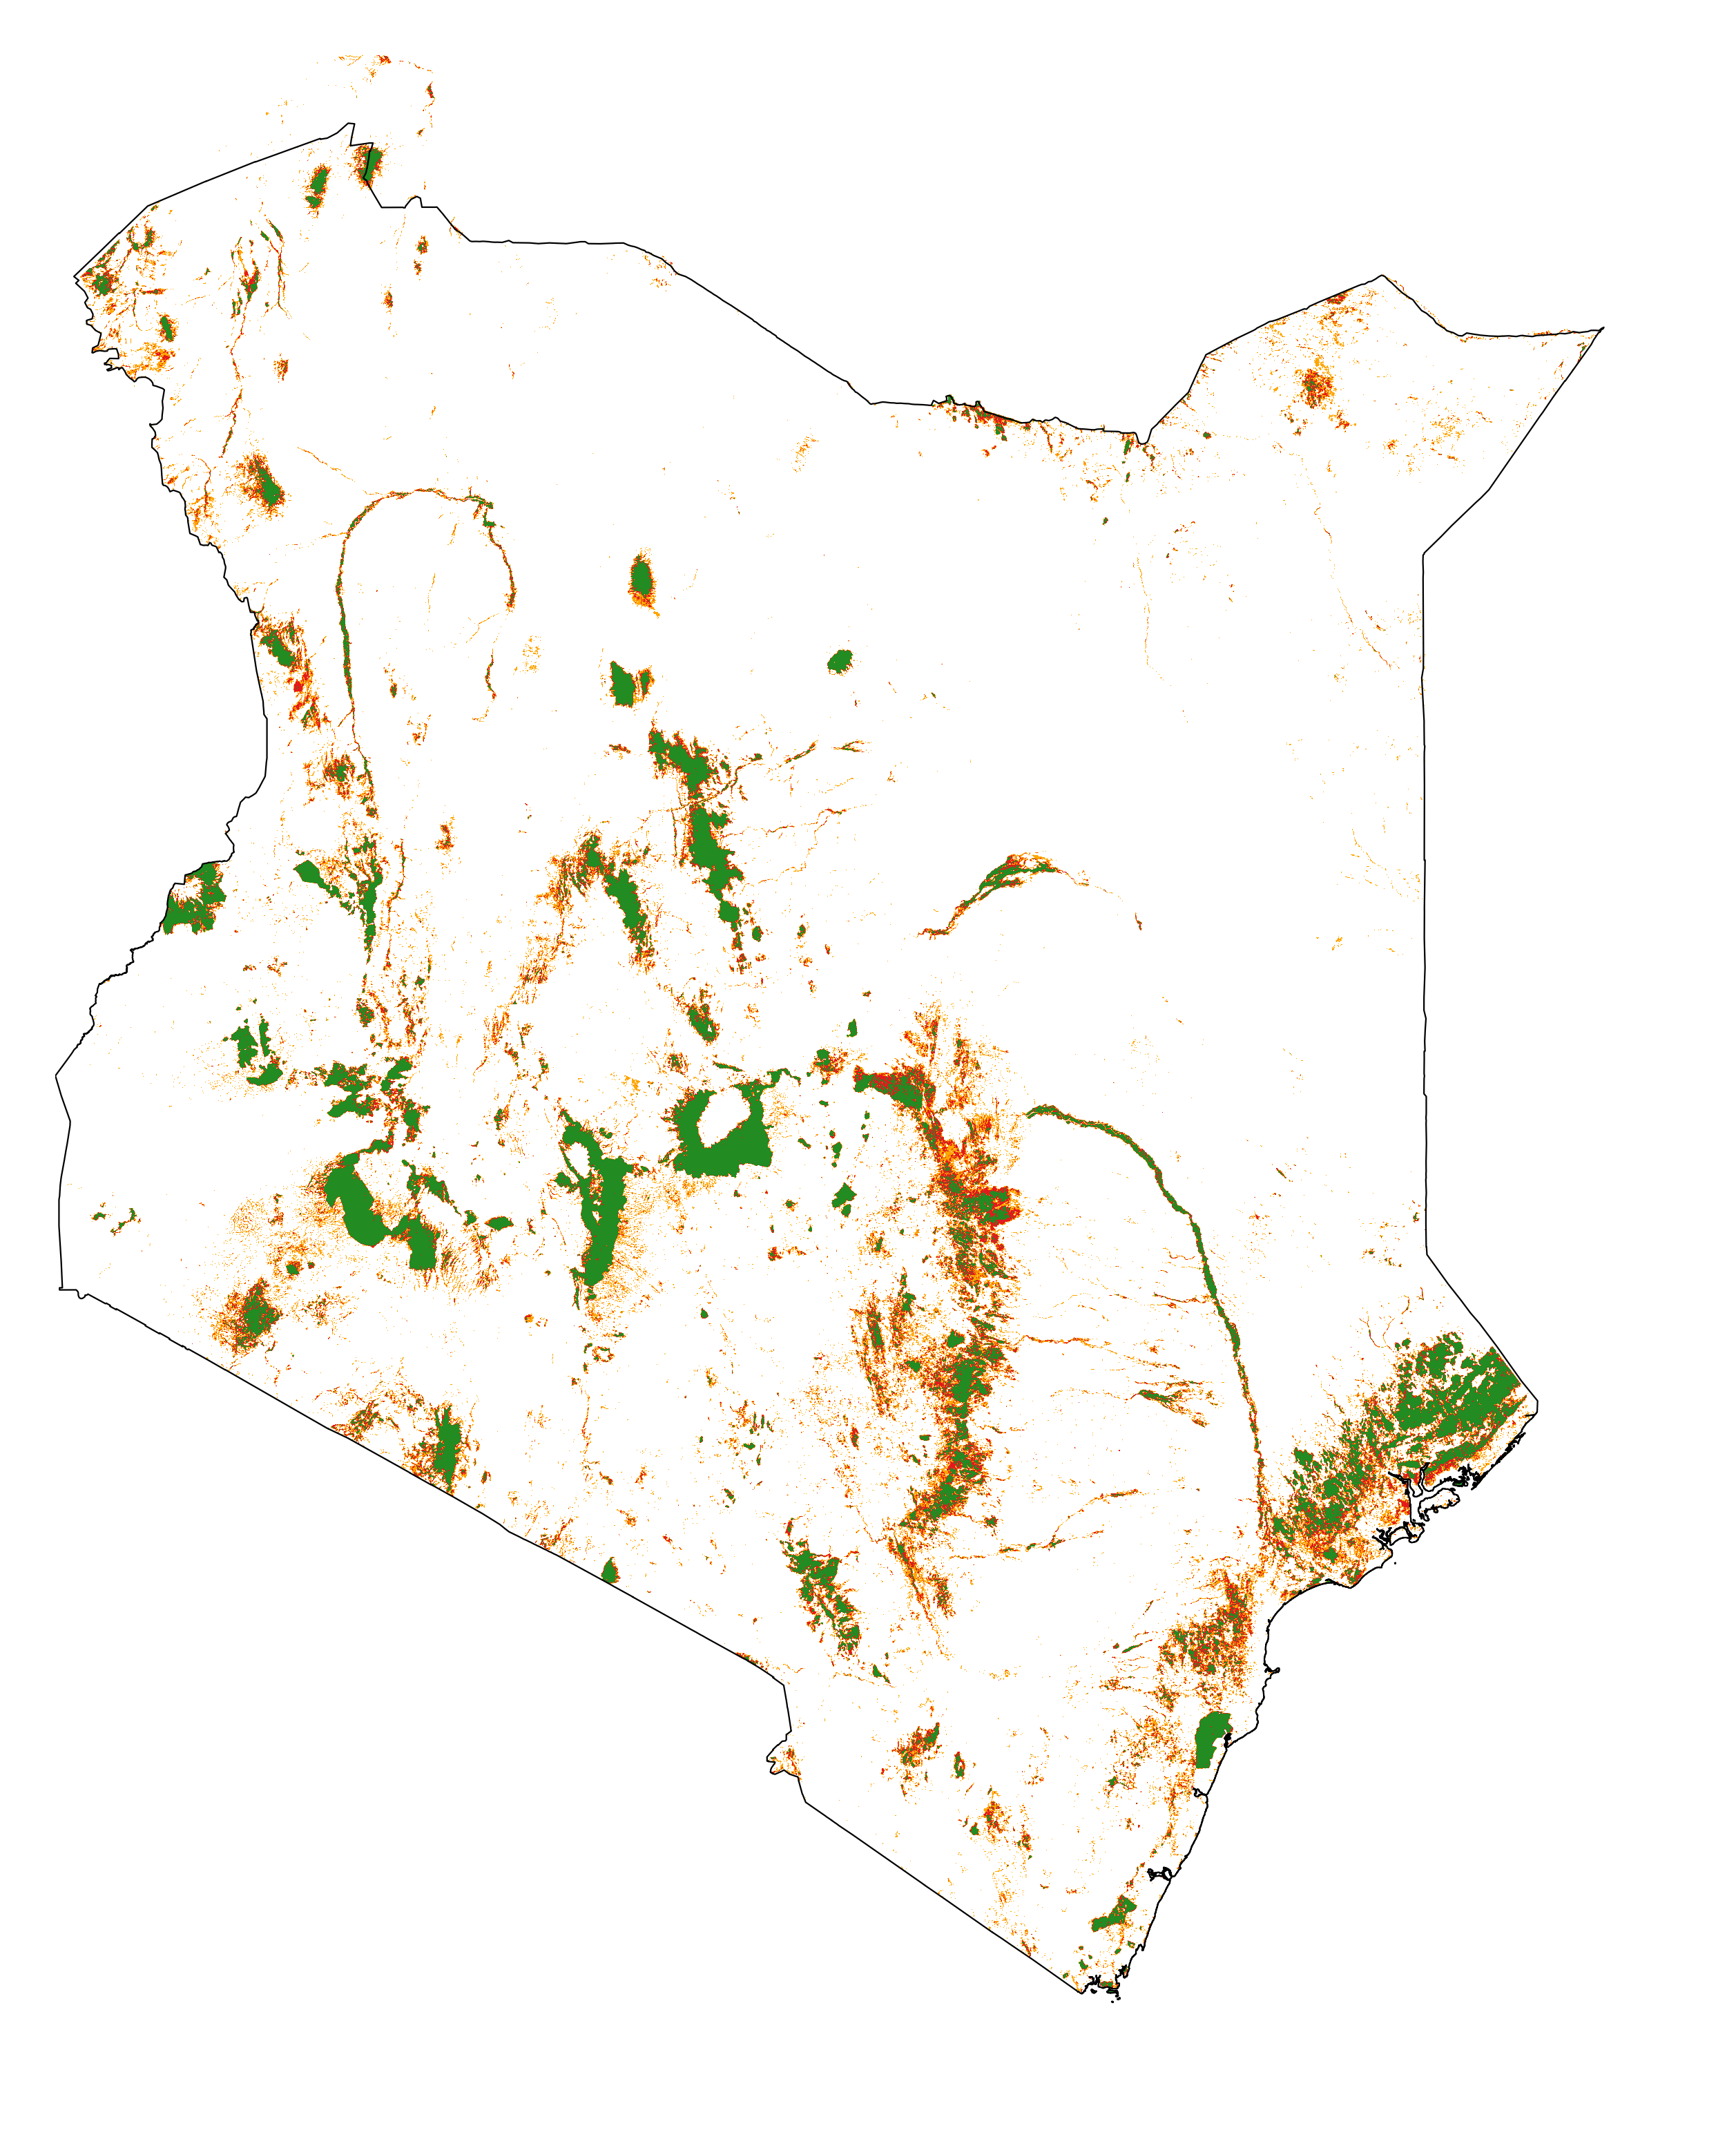
\includegraphics[width=0.8\linewidth]{outputs_kenya/fcc123.png}
\caption{\label{fig:org9213527}\textbf{Forest cover change map.} Deforestation on the first period (2010--2014) is in orange, deforestation on the second period (2014--2018) is in red and remaining forest (in 2018) is in green.}
\end{figure}

\section{Deriving the deforestation risk map}
\label{sec:org07ad532}

We derive the deforestation risk map using the \texttt{makemap()} function. This function calls a sequence of functions from the \texttt{riskmapjnr} package which perform all the steps detailed in the JNR methodology. We can use parallel computing using several CPUs.

\begin{minted}[breaklines=true,bgcolor=bg]{python}
ncpu = mp.cpu_count() - 2
print(f"Number of CPUs: {ncpu}.") 
\end{minted}

\begin{verbatim}
Number of CPUs: 6.
\end{verbatim}


\begin{minted}[breaklines=true,bgcolor=bg]{python}
start_time = time.time()
results_makemap = rmj.makemap(
    fcc_file=fcc_file,
    time_interval=[4, 4],
    output_dir=out_dir,
    clean=False,
    dist_bins=np.arange(0, 1080, step=30),
    win_sizes=np.arange(5, 200, 16),
    ncat=30,
    parallel=True,
    ncpu=ncpu,
    methods=["Equal Interval", "Equal Area"],
    csize=400,  # 12 km
    no_quantity_error=True,
    figsize=(6.4, 4.8),
    dpi=100,
    blk_rows=200,
    verbose=True)
sec_seq = time.time() - start_time
\end{minted}

\begin{minted}[breaklines=true,bgcolor=bg]{python}
print('Computation time:', time.strftime("%H:%M:%S",time.gmtime(sec_seq)))
\end{minted}

\begin{verbatim}
Computation time: 00:38:44
\end{verbatim}

\section{Results}
\label{sec:orgcaa4918}

\subsection{Deforestation risk and distance to forest edge}
\label{sec:orgfd3040e}

We obtain the threshold for the distance to forest edge beyond which the deforestation risk is negligible.

\begin{minted}[breaklines=true,bgcolor=bg]{python}
dist_thresh = results_makemap["dist_thresh"]
print(f"The distance theshold is {dist_thresh} m.")
\end{minted}

\begin{verbatim}
The distance theshold is 780 m.
\end{verbatim}


We have access to a table indicating the cumulative percentage of deforestation as a function of the distance to forest edge.

\begin{center}
\begin{tabular}{rrrrr}
Distance & Npixels & Area & Cumulation & Percentage\\
\hline
30 & 1.4005e+07 & 1.26045e+06 & 1.26045e+06 & 48.9547\\
60 & 5.35311e+06 & 481780 & 1.74223e+06 & 67.6666\\
90 & 3.02736e+06 & 272463 & 2.01469e+06 & 78.2489\\
120 & 1.49449e+06 & 134504 & 2.1492e+06 & 83.4729\\
150 & 1.17144e+06 & 105430 & 2.25463e+06 & 87.5677\\
180 & 639743 & 57576.9 & 2.3122e+06 & 89.8039\\
210 & 469736 & 42276.2 & 2.35448e+06 & 91.4459\\
240 & 417499 & 37574.9 & 2.39205e+06 & 92.9053\\
270 & 326224 & 29360.2 & 2.42141e+06 & 94.0456\\
300 & 260730 & 23465.7 & 2.44488e+06 & 94.957\\
330 & 179341 & 16140.7 & 2.46102e+06 & 95.5839\\
360 & 147688 & 13291.9 & 2.47431e+06 & 96.1001\\
390 & 153559 & 13820.3 & 2.48813e+06 & 96.6369\\
420 & 109451 & 9850.59 & 2.49798e+06 & 97.0195\\
450 & 98440 & 8859.6 & 2.50684e+06 & 97.3636\\
480 & 72145 & 6493.05 & 2.51334e+06 & 97.6158\\
510 & 70682 & 6361.38 & 2.5197e+06 & 97.8628\\
540 & 58834 & 5295.06 & 2.52499e+06 & 98.0685\\
570 & 53707 & 4833.63 & 2.52983e+06 & 98.2562\\
600 & 47735 & 4296.15 & 2.53412e+06 & 98.4231\\
630 & 36436 & 3279.24 & 2.5374e+06 & 98.5504\\
660 & 38346 & 3451.14 & 2.54085e+06 & 98.6845\\
690 & 30219 & 2719.71 & 2.54357e+06 & 98.7901\\
720 & 26853 & 2416.77 & 2.54599e+06 & 98.884\\
750 & 27575 & 2481.75 & 2.54847e+06 & 98.9804\\
780 & 22398 & 2015.82 & 2.55049e+06 & 99.0586\\
810 & 20402 & 1836.18 & 2.55232e+06 & 99.13\\
840 & 17439 & 1569.51 & 2.55389e+06 & 99.1909\\
870 & 16532 & 1487.88 & 2.55538e+06 & 99.2487\\
900 & 17080 & 1537.2 & 2.55692e+06 & 99.3084\\
\end{tabular}
\end{center}

We also have access to a plot showing how the cumulative percentage of deforestation increases with the distance to forest edge.

\begin{minted}[breaklines=true,bgcolor=bg]{python}
os.path.join(out_dir, "perc_dist.png")
\end{minted}

\begin{figure}[H]
\centering
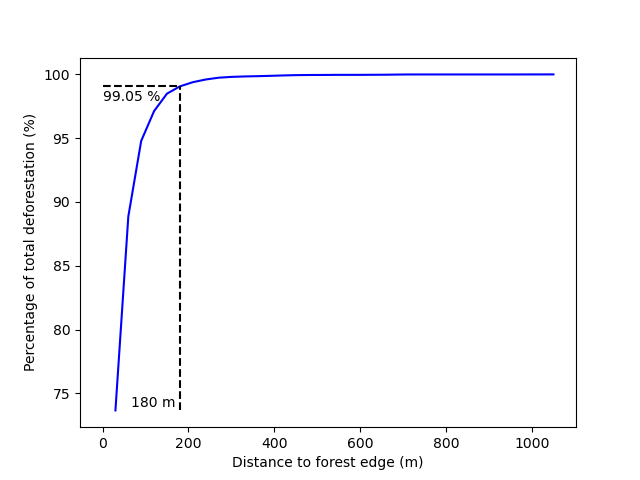
\includegraphics[width=0.8\linewidth]{outputs_kenya/perc_dist.png}
\caption{\label{fig:org77c5a1c}\textbf{Identifying areas for which the risk of deforestation is negligible.} Figure shows that more than 99\% of the deforestation occurs within a distance from the forest edge ≤ 180 m. Forest areas located at a distance > 180 m from the forest edge can be considered as having no risk of being deforested.}
\end{figure}

\subsection{Best model}
\label{sec:orga10423d}

We can plot the change in wRMSE value with both the window size and slicing algorithm. It seems that the ``Equal Interval'' (ei) algorithm provides lower wRMSE values. The lowest wRMSE value is obtained for a window size between 25 and 50 pixels.

\begin{minted}[breaklines=true,bgcolor=bg]{python}
os.path.join(out_dir, "map_comp.png")
\end{minted}

\begin{figure}[H]
\centering
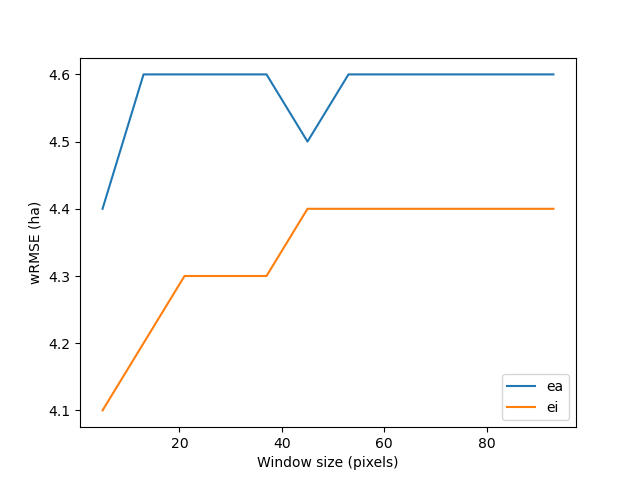
\includegraphics[width=0.8\linewidth]{outputs_kenya/map_comp.png}
\caption{\label{fig:org834d205}\textbf{Change in wRMSE values as a function of both window size and slicing algorithm}. ``ei'' is the ``Equal Interval'' algorithm and ``ea'' is the ``Equal Area'' algorithm.}
\end{figure}

We identify the moving window size and the slicing algorithm of the best model.

\begin{minted}[breaklines=true,bgcolor=bg]{python}
ws_hat = results_makemap["ws_hat"]
m_hat = results_makemap["m_hat"]
print(f"The best moving window size is {ws_hat} pixels.")
print(f"The best slicing algorithm is '{m_hat}'.")
\end{minted}

\begin{verbatim}
The best moving window size is 37 pixels.
The best slicing algorithm is 'ei'.
\end{verbatim}

\subsection{Validation}
\label{sec:org4d1246f}

\begin{minted}[breaklines=true,bgcolor=bg]{python}
os.path.join(out_dir, f"pred_obs_ws{ws_hat}_{m_hat}.png")
\end{minted}

\begin{figure}[H]
\centering
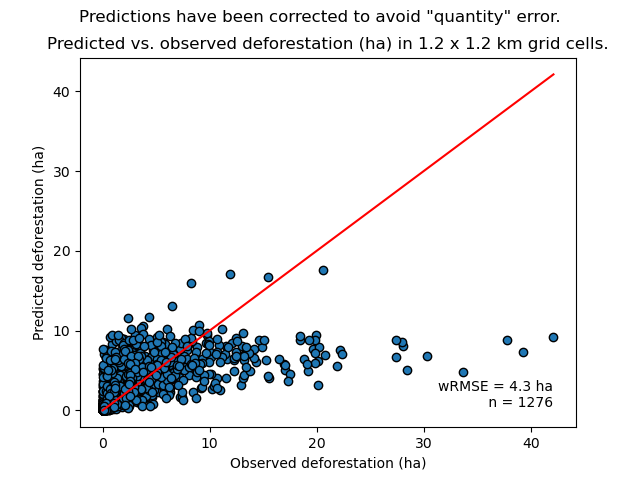
\includegraphics[width=0.8\linewidth]{outputs_kenya/pred_obs_ws37_ei.png}
\caption{\label{fig:org8f8f1c2}\textbf{Relationship between observed and predicted deforestation in 1 x 1 km grid cells for the best model}. The red line is the identity line. Values of the weighted root mean squared error (wRMSE, in ha) and of the number of observations (\(n\), the number of spatial cells) are reported on the graph.}
\end{figure}

\subsection{Risk map of deforestation}
\label{sec:org4f408e2}

We plot the risk map using the \texttt{plot.riskmap()} function.

\begin{minted}[breaklines=true,bgcolor=bg]{python}
ifile = os.path.join(out_dir, f"riskmap_ws{ws_hat}_{m_hat}.tif")
ofile = os.path.join(out_dir, f"riskmap_ws{ws_hat}_{m_hat}.png")
riskmap_fig = rmj.plot.riskmap(
    input_risk_map=ifile,
    maxpixels=1e8,
    output_file=ofile,
    borders=border_file,
    legend=True,
    figsize=(5, 4), dpi=800, linewidth=0.2,)
ofile
\end{minted}

\begin{figure}[H]
\centering
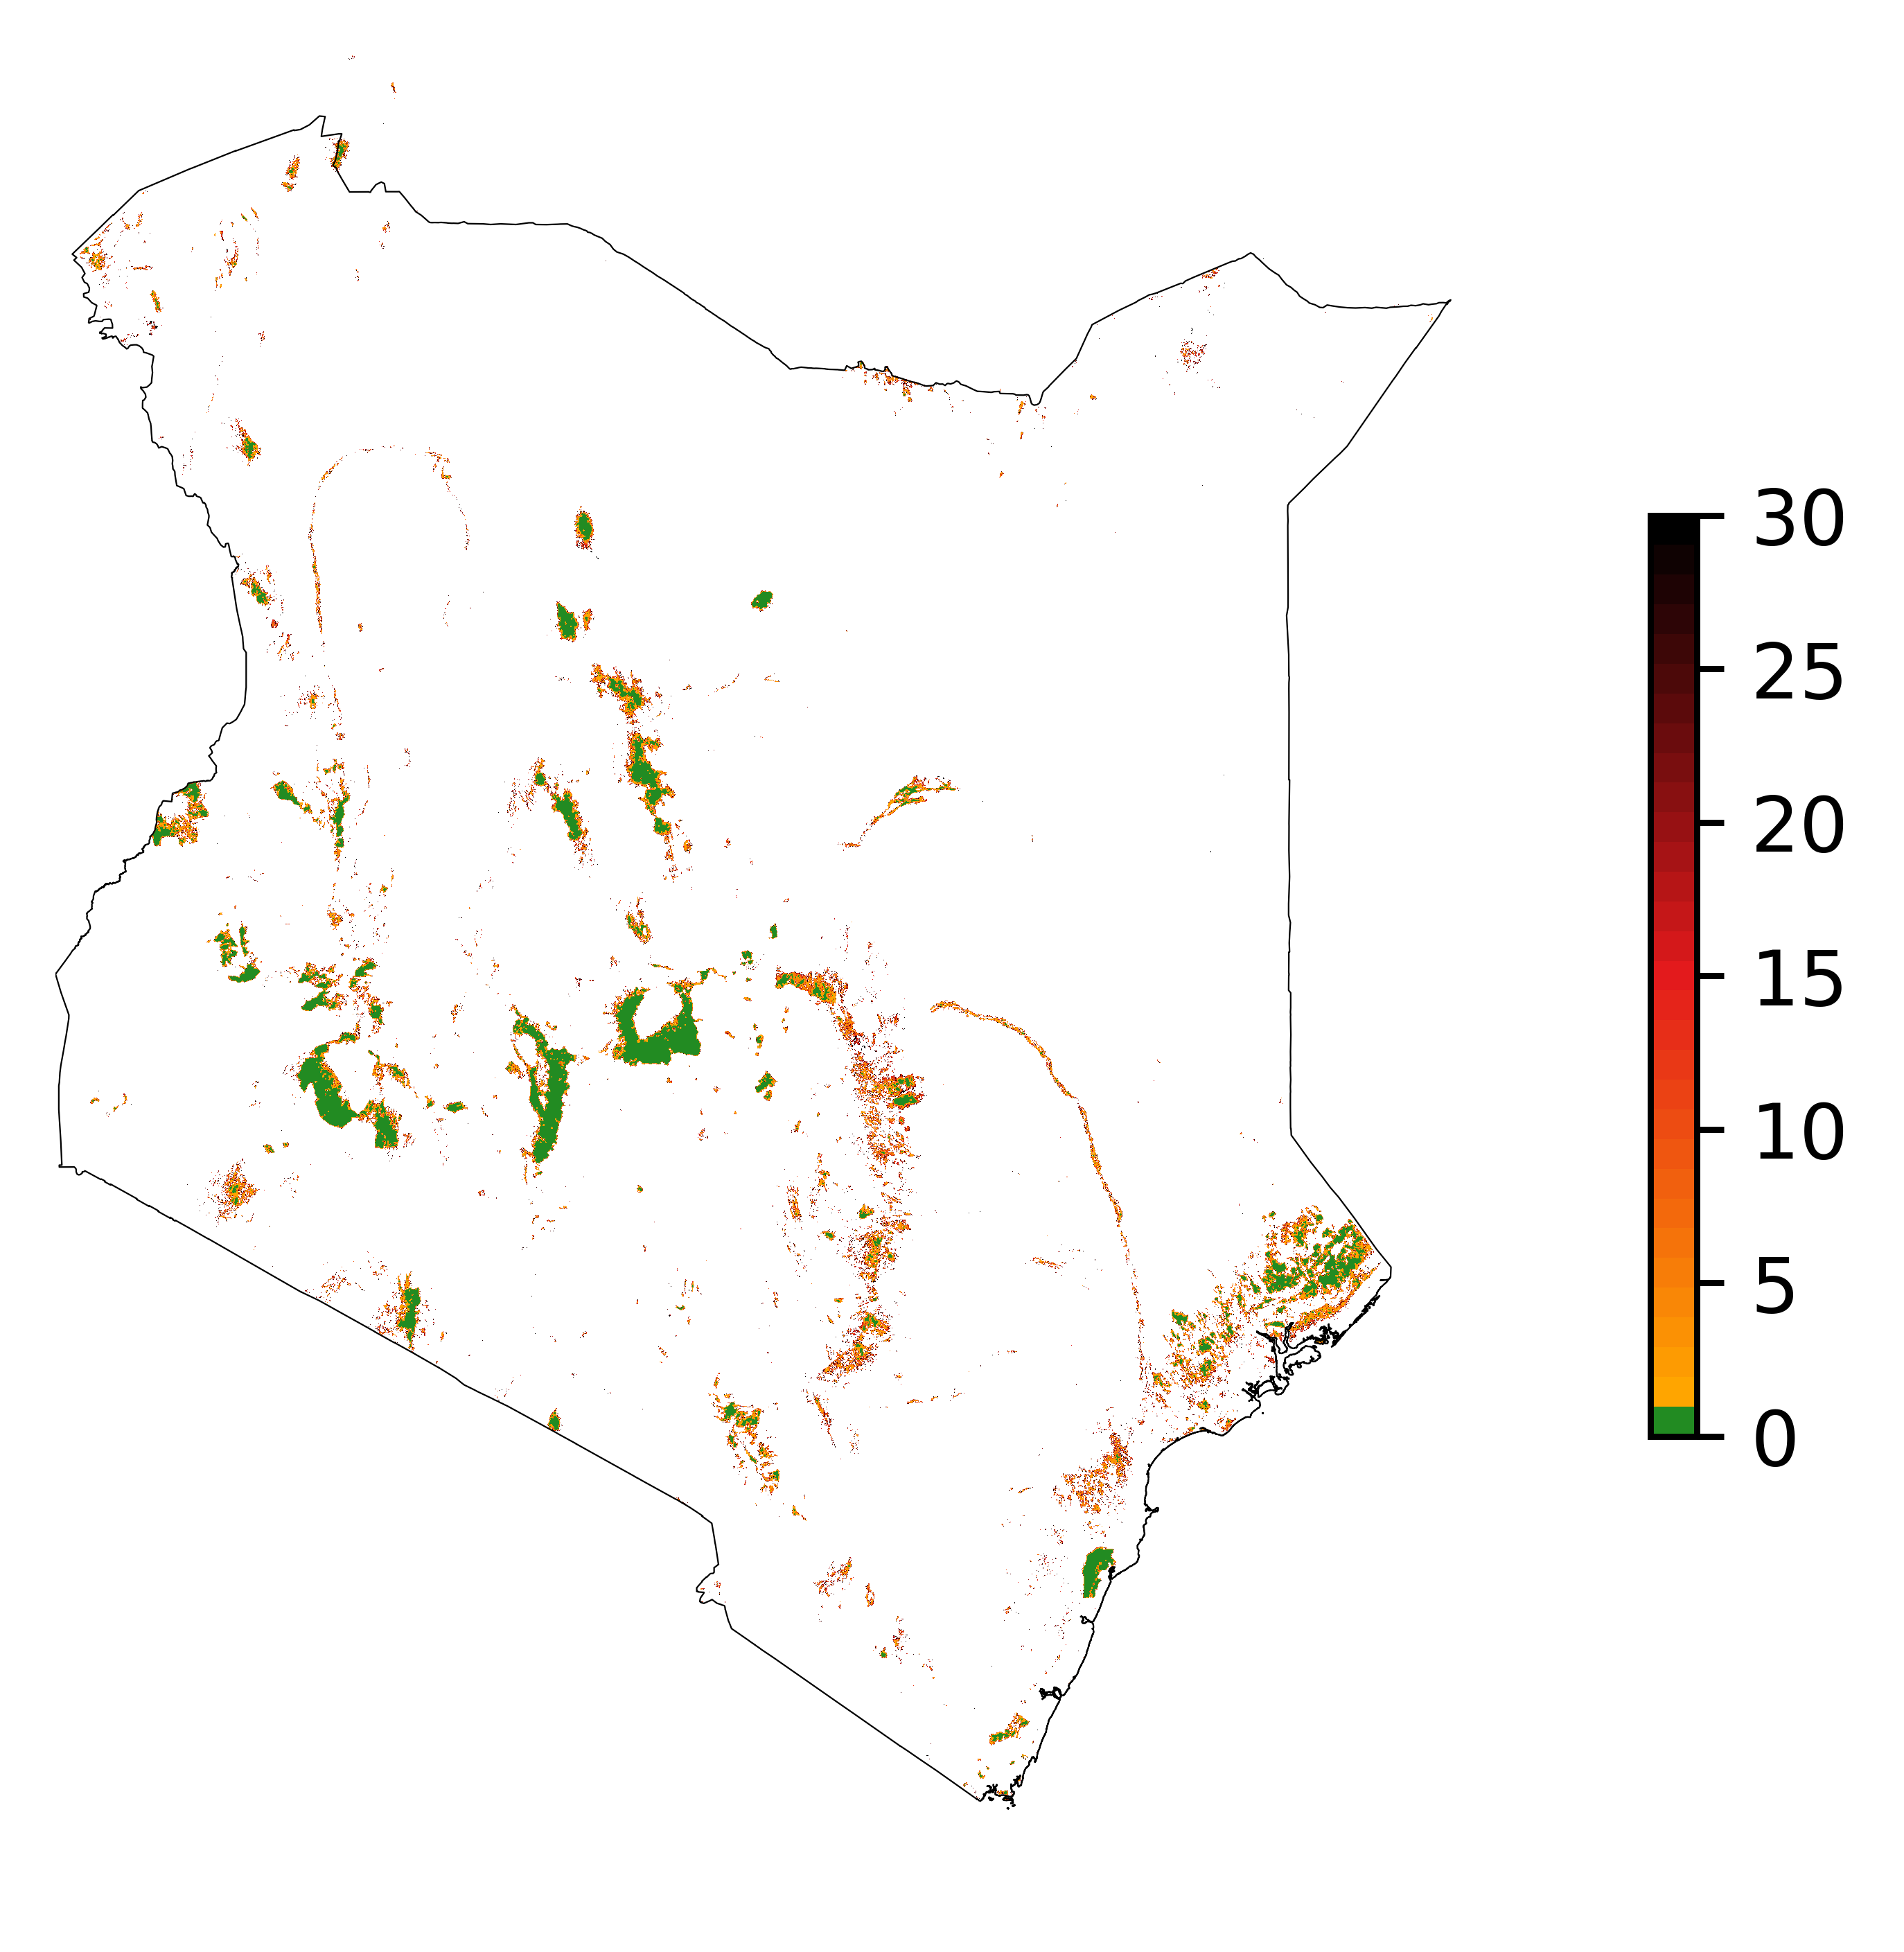
\includegraphics[width=0.8\linewidth]{outputs_kenya/riskmap_ws37_ei.png}
\caption{\label{fig:org1f66a0c}\textbf{Map of the deforestation risk following the JNR methodology}. Forest pixels are categorized in up to 30 classes of deforestation risk. Forest pixels which belong to the class 0 (in green) are located farther than a distance of 780 m from the forest edge and have a negligible risk of being deforested.}
\end{figure}

\section{Conclusion}
\label{sec:orga9059fc}

We have presented the use of the \texttt{riskmapjnr} Python package to obtain a map of the deforestation risk following the JNR methodology. As said previously, the JNR methodology is currently being discussed and will likely be subject to changes. The first results we have obtained applying the JNR methodology to a small-scale study area allow us to make some recommendations regarding how the JNR methodology could be improved to obtain an accurate map of the deforestation risk.

\section{References}
\label{sec:org23ddb58}

\begin{hangparas}{1.5em}{1}

\end{hangparas}
\end{document}